\chapter{Wolterミラーの誤差応答シミュレーション}
\thispagestyle{empty}
\label{chap2}
\graphicspath{{chap2/figure/}}
\minitoc

\newpage
%%%%%%%%%%%%%%%%%%%%%%%%%%%%%%%%%%%%%%%%%%%%%%%%%%%%%%%%%%%%%%%%%%%%%%%%%%%%%


% ================================================== %
% section
% ================================================== %
\section{諸言}
\label{chap2_introduction}

Wolterミラーを光学系に組み込んで利用する際、加工時の誤差および設置時の誤差によってその理想の集光・結像が損なわれる。
設置時に生じる位置や姿勢の誤差は利用する前に校正することが出来るため、Wolterミラー開発段階において注目するべきは製造時に発生する形状誤差である。
ミラー製造プロセスにおける重篤な問題点を指摘し改善に繋げるためには、Wolterミラーが十分な性能を発揮するために必要な加工精度を調べ、実際に計測された結果と比較する必要がある。
そこで、本章ではまず、ミラー表面の形状誤差入力に対する集光面波動場の応答をシミュレーションによって解析し、種々の形状誤差の許容値を計算する。
このシミュレーションは実際にWolterミラーが利用される際に対象となる波長域のX線を光源として行う。
続いて、可視光光源を用いた測定装置によってこれらの許容誤差と実際のミラーに存在する誤差量の比較を行うためには、どのような測定仕様を満たす必要があるかを調べる。
最後に、それぞれの誤差が与える波面誤差分布をZernike多項式によって近似し、\ref{chap3}章以降で行われる位相回復計算の結果を解析するための基底情報として与える。

\clearpage
% ================================================== %
% section
% ================================================== %
\newpage
\section{誤差の評価と許容される誤差}
\label{chap2_beam_evaluation_standard}

理想の集光波面との差異を定量的に評価するためには、具体的な評価軸が必要である。
そこで主に用いられるのが、Strehl比、HPD、FWHMの3つの特徴量である。

\subsection{Strehl比}
\label{chap2_strehl_ratio}
主に集光光学系の文脈において、理想の集光状態を「回折限界集光」と呼ぶ。
回折限界集光の状態にあるかどうかを判別する1つの指標として用いられるのが、Strehl比である。
Strehl比とは、実際の集光波面における最大値と回折限界時の集光波面における最大値の比として定義される。
つまり、振幅を$I(\mathbf{r})$として

\[
r_{\mathrm{Strehl}} = \frac{ \max{\sqrt{I(\mathbf{r})} } }{ \max{ \sqrt{I_{\mathrm{ideal}}( \mathbf{r} )} } }
\]

と定まる。
図\ref{fig:strehl_explanation}にその模式的なグラフを示す。
Strehl比を評価する基準として、Marechal基準\cite{BornWolf:1999:Book}が知られている。
Marechal基準では、Strehl比が0.8以上であるときその系は回折限界集光をしている、とする。
この0.8という値には体系的な根拠はなく、解析・実験における経験的な指標として扱われている。
本論文では、この慣例を踏襲し、0.8を閾値としてStrehl比を評価する。

\begin{figure}[h]
\centering
\includegraphics[width=10cm]{strehl.png}
\caption{Strehl比計算の模式図}
\label{fig:strehl_explanation}
\end{figure}

\subsection{HPD (Half Power Diameter)}
\label{chap2_hpd}

Strehl比による比較検討では「回折限界集光をしているか」に主眼を置いているが、天文用Wolterミラーのように達成すべき角度分解能が決まっている場合では、直接その分解能要求を満たしているかどうかを判定するのが実用的である。
分解能を決定するのは、焦点面におけるビームの集光サイズであり、これは大きく2つの定義によって議論される。
1つが、Half Power Diameter(HPD)である。
HPDは「焦点面上の全強度の50\%の強度を含む円の直径」と定義される。
つまり、
\[
    \sum_{d\leq d_{\mathrm{HPD}}} \sqrt{ I(\mathbf{r}) } = \frac{1}{2} \sum \sqrt{ I(\mathbf{r}) }
\]
を満たすような直径$d_{\mathrm{HPD}}$として定義される。
図\ref{fig:hpd_explanation}にその例を示す。
この赤円の内側の強度総和値は、全体の強度総和値の半分になっている。

\begin{figure}[!ht]
\centering
\includegraphics[width=6cm]{HPD.png}
\caption{HPDの例}
\label{fig:hpd_explanation}
\end{figure}

あるHPDを持つようなのふたつの結像点を分離できるような限界の配置が図\ref{fig:hpd_resolution_limit}のときであるとするならば、0.5秒角分解能という達成目標は図\ref{fig:hpd_arcsecond}が示すようなHPDで言い換えることができる。
つまり、ミラー上流端中心から半径を見込む角度がちょうど0.5秒角となるようなHPDが達成目標となる。
具体的には、ミラー上流端開口から焦点面までの距離2.1025 mに対してHPDは\SI{10.19}{\micro \metre}と計算される。
HPDを指標とした評価では、これを基準とする。

\begin{figure}[ht]
\centering
\includegraphics[width=6cm]{hpd_resolution_limit.png}
\caption{解像限界の図}
\label{fig:hpd_resolution_limit}
\end{figure}

\begin{figure}[ht]
\centering
\includegraphics[width=12cm]{hpd_arcsecond.png}
\caption{HPDと結像分解能の関係}
\label{fig:hpd_arcsecond}
\end{figure}


\subsection{FWHM (Full Width Half Maximum)}
\label{chap2_fwhm}

HPDに並んでビーム集光サイズの評価として用いられるのが、FWHM(Full Width Half Maximum)である。
こちらは焦点面を集光点を通る直線によって切断したプロファイルに対して、「焦点面における最大値の半分の値を取る2点の距離」と定められる。
図\ref{fig:fwhm_explanation_profile}は1つのプロファイルに対するFWHMの例である。
切断する直線には任意性があるため、通常は図\ref{fig:fwhm_explanation}のように水平方向と鉛直方向の2方向に関して切断しこれを評価する。
\ref{chap2_ideal_focusing}節で具体的な計算例を示すが、結像性能の強いWolterミラーはメインピークに対して比較的大きいサブピークが細かく連なるような集光面強度分布を持つ。
そのため、強度はメインピークより外側に広がって存在しており、解像限界を決める上ではHPDの方が適していると言える。
FWHMはミラー開発の目標に対する評価ではなく、本研究中でのパラメータ設定の指標として用いることとする。

\begin{figure}[ht]
\centering
\includegraphics[width=8cm]{FWHM.png}
\caption{FWHMの例}
\label{fig:fwhm_explanation_profile}
\end{figure}

\begin{figure}[!ht]
\centering

\subfloat[horizontal]{
    \includegraphics[width=5cm]{FWHM_horizontal.png}
    \label{fig:fwhm_explanation_horizontal}
}
\subfloat[vertical]{
    \centering
    \includegraphics[width=5cm]{FWHM_vertical.png}
    \label{fig:fwhm_explanation_vertical}
}
\caption[]{切断の例 水平:\subref{fig:fwhm_explanation_horizontal}, 鉛直:\subref{fig:fwhm_explanation_vertical}}
\label{fig:fwhm_explanation}
\end{figure}


\clearpage
% ================================================== %
% section
% ================================================== %
\newpage

\section{Wolterミラーにおける光学波動場の伝播}
\label{chap2_wolter_diffraction_apporoximation}

シミュレーションおよび位相回復計算を行うにあたり、測定対象のWolterミラーの光学系において適用するべき波動場伝播の近似公式について検討する。
光学波動場の伝播に関しての詳細は付録において解説する。
まず、1章\ref{chap1_wolter_arrangement}節で示したパラメータについて、Fresnel回折近似の成立条件が成り立っているかどうかを確認する。
Fresnel回折近似が成り立つための条件は、近似で切り捨てる微小項が1 radより十分小さいときであり、これは式\ref{eqn:fresnel_approximation_condition}で表される。
ただし$z$は伝搬距離、$\lambda$は波長、$(x, y), (\xi, \eta)$は実空間および逆空間の座標を表す。

\begin{equation}
\label{eqn:fresnel_approximation_condition}
    \frac{\pi}{4\lambda} \max \left\{ (x-\xi)^2 + (y-\eta)^2 \right\}^2 / z^3 \ll 1
\end{equation}

焦点面の大きさを測定実験に用いるディテクタと同じ 36.9 mm $\times$ 36.9 mm として近似条件を計算すると、左辺の値は 1.645 radとなった。
これは 1 rad に対して十分小さいとは言えず、Fresnel回折近似条件を満たさない。
しかし、Fresnel回折近似を満たしていない場合でも、計算を進めていく上でそれがほとんど影響を及ぼさない場合がある。
位相回復計算においては数万回の伝搬計算を行うため、1回のコストは最小限であることが好ましい。
そこで、厳密計算であるRayleigh-Sommerfeld回折積分とFresnel回折積分近似の集光面強度分布を比較し、実用上の問題が存在するかどうかを検討する。
まず、表\ref{tb:check_approximation_validity_1}に示すような適当な分割で回折積分を実行し、集光波面分布におけるメインピークのFWHMを調べる。

\begin{table}[!ht]
\begin{center}
  \caption{Fresnel回折近似適用可能性の検討1}
  \begin{tabular}{|c|c|} \hline
    項目 & 値 \\ \hline
    波長 & 632.8 nm \\
    画素数 & $2048 \times 2048$ \\
    焦点面ピクセルサイズ & \SI{5.0}{\micro \metre} \\ \hline
  \end{tabular}
  \label{tb:check_approximation_validity_1}
\end{center}
\end{table}

計算の結果、プロファイルは図\ref{fig:fwhm_approximation}のようになった。

\begin{figure}[ht]
\centering
\includegraphics[width=8cm]{../../chap2/figure/fwhm_approximation.png}
\caption{回折積分計算による簡易的な計算で得られた焦点面強度プロファイル}
\label{fig:fwhm_approximation}
\end{figure}

ここから計算されるFWHMは4ピクセル分の\SI{20}{\micro \metre}であった。
これを踏まえ、メインピークを十分な分割数で観察できるよう焦点面ピクセルサイズが\SI{1}{\micro \metre}になるような表\ref{tb:check_approximation_validity_2}のパラメータで回折積分およびFresnel回折近似を用いた場合の集光面強度プロファイルを計算し、比較を行う。

\begin{table}[!ht]
\begin{center}
  \caption{Fresnel回折近似適用可能性の検討2}
  \begin{tabular}{|c|c|} \hline
    項目 & 値 \\ \hline
    波長 & 632.8 nm \\
    画素数 & $4096 \times 4096$ \\
    焦点面ピクセルサイズ & \SI{1.0}{\micro \metre} \\ \hline
  \end{tabular}
  \label{tb:check_approximation_validity_2}
\end{center}
\end{table}

計算の結果、プロファイルは図\ref{fig:diffraction_comparison}のようになった。
また、2つのプロファイルの差分を取って回折積分の最大値で規格化したグラフが図\ref{fig:diffraction_comparison_normalized_diff}である。

\begin{figure}[!ht]
\centering

\subfloat[プロファイルプロット]{
    \includegraphics[width=6cm]{../../chap2/figure/diffraction_comparison_profile.png}
    \label{fig:diffraction_comparison_profile}
}
\subfloat[規格化されたプロファイル誤差]{
    \centering
    \includegraphics[width=6cm]{../../chap2/figure/diffraction_comparison_normalized_diff.png}
    \label{fig:diffraction_comparison_normalized_diff}
}

\caption[]{Rayleigh-Sommerfeld回折積分とFresnel回折積分のプロファイル比較}
\label{fig:diffraction_comparison}
\end{figure}

差分の絶対値の最大値は0.00242程度となった。
これは十分小さく、実際の計測で生じうるノイズと同程度以下であるため、シミュレーションでの検討および位相回復計算を行う上で致命的な問題をもたらさない。
ゆえに、以降の伝搬計算はFresnel回折近似を用いて行う。


\clearpage
% ================================================== %
% section
% ================================================== %
\newpage


\section{シミュレーションの方法}
\label{chap2_simulation_methodology}

誤差応答シミュレーションは、図\ref{fig:simulation_schematic}に示すように、下流端面における波動場を求め、それを焦点面に伝播するという流れで行われる。
多数の条件に対し効率よくシミュレーションを行うため、下流端面上の波動場を幾何光学に基づく光線追跡法によって計算し、また下流端面から焦点面への伝播は\ref{chap2_wolter_diffraction_apporoximation}節に述べたようにFresnel回折近似を用いて計算する。

\begin{figure}[h]
\centering
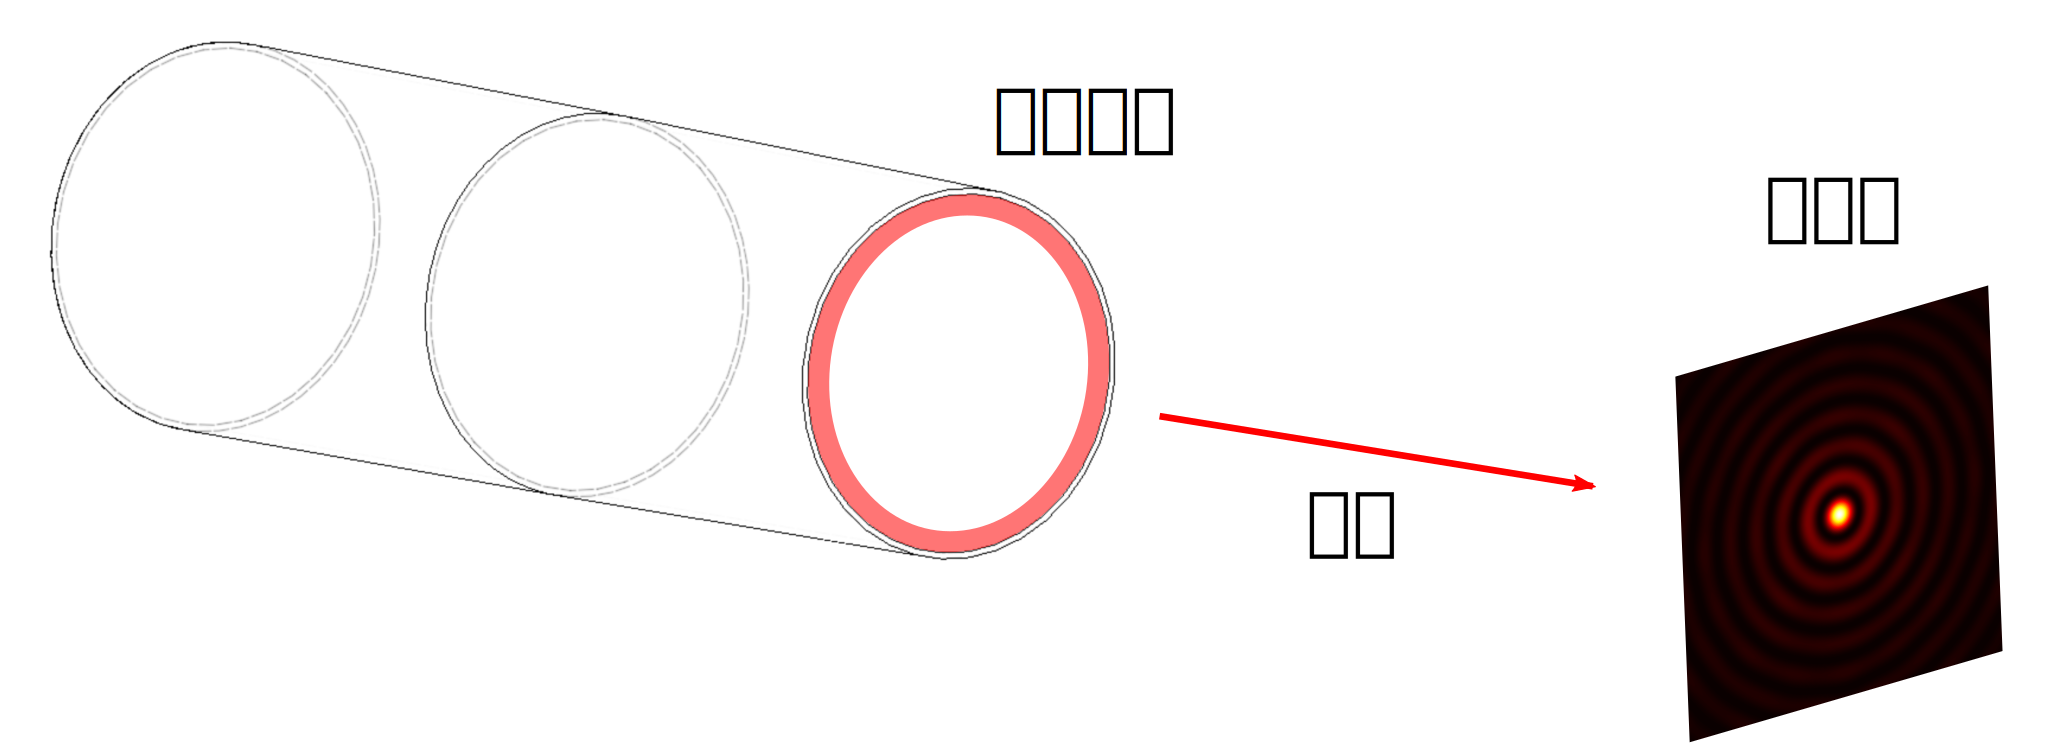
\includegraphics[width=12cm]{method/simulation_schematic.png}
\caption{シミュレーションの概観}
\label{fig:simulation_schematic}
\end{figure}

以下に具体的なシミュレーションの手順を示す。

\begin{enumerate}[\expandafter\maru 1]
  \item 放物面および双曲面について、ミラー表面の表現$f(x, y, z)=0$を与える。
    理想形状のミラーの場合、これは具体的に式\ref{eqn:parabola_surface_func}および式\ref{eqn:parabola_surface_func}のように与えられる。 \\
    \begin{eqnarray}
        f_p(x, y, z) &=& x^2 + y^2 - \left|4p(z-p-f2)\right| = 0 \label{eqn:parabola_surface_func} \\
        f_h(x, y, z) &=& \frac{\left(z - \frac{(f1 + f2)}{2}\right)^2}{a^2} - \frac{x^2 + y^2}{b^2} - 1 = 0 \label{eqn:hyperbola_surface_func}
    \end{eqnarray}
  \item 図\ref{fig:simulation_raytrace}に示すように、ミラー下流端面を$N \times N$のピクセルに分割する。
    下流端面上の集光ビーム定義域に含まれる全てのピクセルについて、光線追跡によって以下の手順で光路長を計算する。
    \begin{enumerate}[(1)]
      \item 下流端面上の点を$P_k$とする。
        誤差のない理想形状のミラーによって2回の反射の後に$P_k$に到達するような入射光線$\mathbf{i}_{k,0}$を求める。
        具体的には、焦点を始点として集光ビームの進行方向と逆向きに辿る、つまり焦点からPに向かう光線を双曲面、放物面の順に反射すれば、得られた光線が入射光線となる。
        反射の計算について、反射点は光線と\expandafter\maru 1 で与えた$f(x, y, z)=0$との交点として、また反射光の向きは反射の法則から$\mathbf{v}_{\text{ref}} = \mathbf{v}_{\text{in}} + 2 (-\mathbf{v}_{\text{in}} \cdot \mathbf{n}) \mathbf{n}$として計算できる。
      \item 求めた入射光線$\mathbf{i}_{k,0}$を初期値として光線位置を$x, y$方向に動かして最適化し、誤差を入力したミラーにおける入射光線$\mathbf{i}_k$を求める。
        最適化の計算はBroyden法で行う。
        入射光$\mathbf{i}_k$から計算される2回反射後の下流端面上の位置$P_k'$と$P_k$の位置誤差$\mathbf{E}=\mathbf{P}_k' - \mathbf{P}_k$に対し、$\mathbf{E}=\mathbf{0}$を入射光線の位置$(x, y)$について解けばよい。
        図\ref{fig:simulation_backtrace}に示すように、入射光線位置$(x, y)$を通る$z$軸に平行な直線として与え、2回反射後の下流端面における目標の点との位置誤差を$\mathbf{0}$に近づけるようにこれを動かす。
      \item 求めた入射光線に対してミラー上流端面から下流端面に至るまでの距離$L$を計算し、点$P$での位相を$k L$(波動場を$\exp(j k L)$)として点$P$に関する計算を終了する。
    \end{enumerate}
  \item 次に、\expandafter\maru 2 で求めた下流端面上の各点$P$に対応する光路から、集光面の光軸方向位置の最適化を行う。
    図\ref{fig:simulation_focal_point_optimize}下流端面から集光点に向かう光線の$z=f$上の分布に対し、重心点と各点の距離の2乗和を$E$とする。
    $E$を最小化するように$f$を変化させることで、収束した$f$と重心点を$G(x_G, y_G)$から焦点位置が$F(x_G, y_G, f)$と定まる。
    初期値には理想の焦点距離$f_1$を与え、最適化は黄金探索によって行う。
  \item 最後に、下流端面から焦点面$z=f$に向かって$(x, y)=(x_G, y_G)$を光軸としてFresnel近似を利用した伝播計算を行う。
\end{enumerate}


\begin{figure}[h]
\centering
\includegraphics[width=10cm]{method/simulation_raytrace_schematic.png}
\caption{光線追跡による下流端面波動場の計算}
\label{fig:simulation_raytrace}
\end{figure}

\begin{figure}[h]
\centering
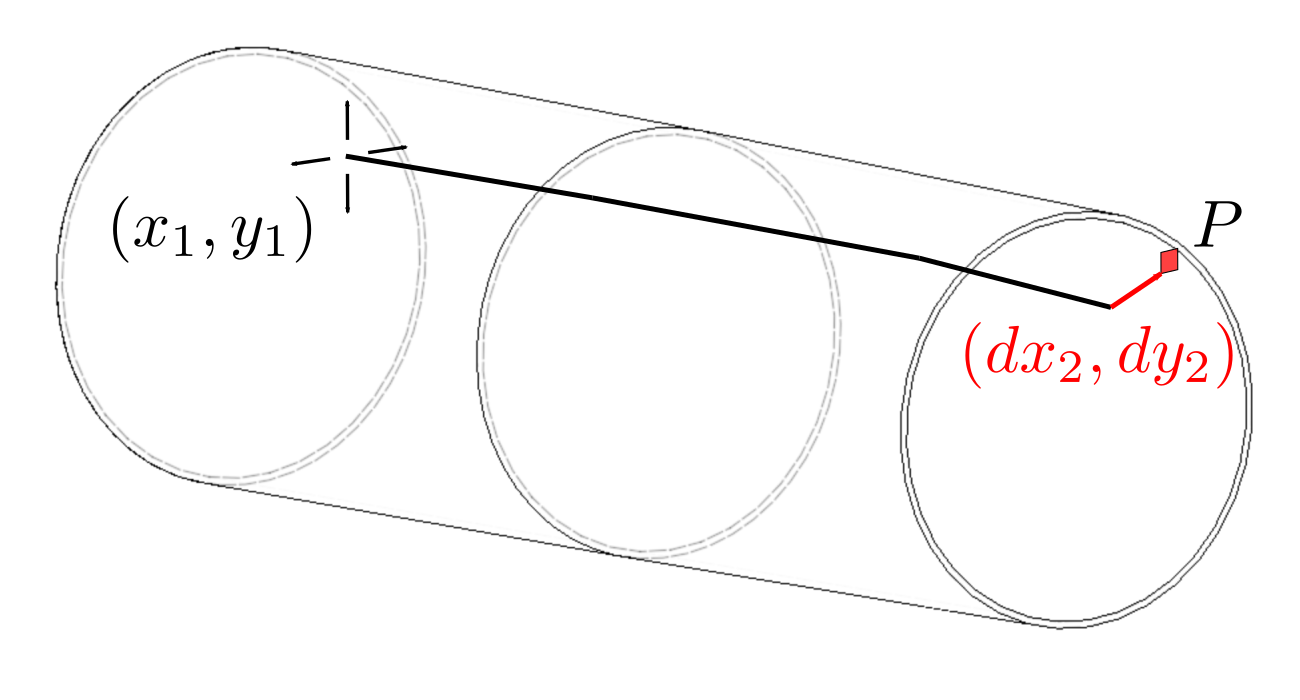
\includegraphics[width=10cm]{method/simulation_backtrace.png}
\caption{点$P$に到達する光路の計算}
\label{fig:simulation_backtrace}
\end{figure}

\begin{figure}[h]
\centering
\includegraphics[width=14cm]{method/simulation_focal_point_optimize.png}
\caption{焦点位置の計算}
\label{fig:simulation_focal_point_optimize}
\end{figure}



\clearpage
% ================================================== %
% section
% ================================================== %
\newpage

\section{計算条件}
\label{chap2_simulation_condition}


\subsection{光源の波長}
\label{chap2_incident_beam_energy}

図\ref{fig:corona_spectrum}は、FOXSI3において撮影されたデータから解析された太陽コロナの活動領域におけるX線スペクトルである。\cite{2019AGUFMSH31C3315V}
これをもとに考えれば、測定対象となるX線のエネルギーは数百 eV から 4 keV程度であることになる。

\begin{figure}[ht]
\centering
\includegraphics[height=4cm]{corona_spectrum.png}
\caption{太陽コロナ活動領域のX線スペクトル\cite{2019AGUFMSH31C3315V}}
\label{fig:corona_spectrum}
\end{figure}

本章では表\ref{tb:simulation_target_energy}に示すように、厳しい形状精度が求められる 4 keV のX線、および\ref{chap5}章の波面計測実験に用いる可視光ビームの波長 632.8 nm を対象にシミュレーションを行う。

\begin{table}[!ht]
\begin{center}
  \caption{シミュレーションで入力する波長・エネルギー}
  \begin{tabular}{|c|c|l|} \hline
    エネルギー & 波長 & 説明 \\ \hline
    4.0 keV & 0.310 nm & 太陽コロナの観測時に対象となるX線 \\
    19.59 eV & 632.8 nm & 可視光計測に用いるHe-Neレーザー \\ \hline
  \end{tabular}
  \label{tb:simulation_target_energy}
\end{center}
\end{table}

\subsection{入力する形状誤差}
\label{chap2_error_input_types}

この節では、入力する形状誤差の種類について述べる。
%まず、形状誤差による波面誤差の線形性について述べておく。
%波面誤差とは、ミラーの形状誤差による光路長の変化量に他ならない。
%平面のミラーで単純化して考えれば、位置

形状誤差は周方向および長手方向の2つの軸で分けて考える。
まず周方向の誤差として、$\Delta r(\theta)=\delta=const$となる(\ref{sub@fig:diameter_error_schematic})直径誤差、および$\Delta r(\theta)=\Delta r_{\mathrm{ideal}}(\theta) + \delta(\theta)$ ($\delta(\theta)$は平均$0$、p-v値が$\delta_{\mathrm{pv}}$の関数)となるような真円度誤差の2種類が存在する。
後者の真円度誤差は周期によって異なる応答が得られるため、代表的な周期として
$sin(2\theta)$で表される(\ref{sub@fig:oval_error_schematic})二山誤差、
周期 $40^\circ$の(\ref{sub@fig:roundness_medium_error_schematic})長周期誤差、
周期 $10^\circ$の(\ref{sub@fig:roundness_medium_error_schematic})中周期誤差、
周期 $1^\circ$の(\ref{sub@fig:roundness_short_error_schematic})短周期誤差
の4つについてそれぞれシミュレーションし、また一定の誤差量に対して周期を変化させた場合のStrehl比およびHPDの変化について調べる。

続いて、長手方向の誤差として、
斜入射角が一定量ずれる(\ref{sub@fig:diameter_error_schematic})テーパ角誤差、
光軸が電鋳時にたわむことで生じる(\ref{sub@fig:axis_deflection_schematic})光軸たわみ、
および平均$0$の凹凸が生じる長手方向プロファイル誤差がある。
プロファイル誤差は真円度誤差と同様に異なる3つの周期
周期 100 mm の(\ref{sub@fig:profile_medium_error_schematic})長周期誤差、
周期 10 mm の(\ref{sub@fig:profile_medium_error_schematic})中周期誤差、
周期 1 mm の(\ref{sub@fig:profile_short_error_schematic})短周期誤差
についてそれぞれシミュレーションし、また一定の誤差量に対して周期を変化させた場合についても調べる。


\begin{figure}[!ht]
\centering

\subfloat[直径誤差]{
    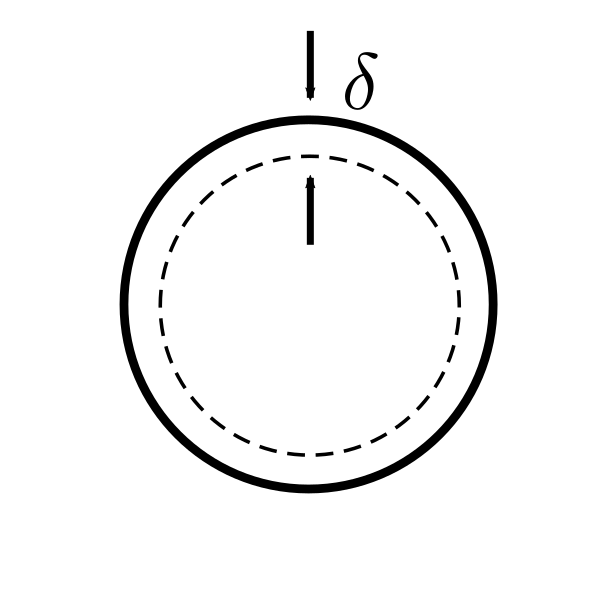
\includegraphics[height=3cm]{error_types/diameter_error_schematic.png}
    \label{fig:diameter_error_schematic}
}
\hspace{5mm}
\subfloat[周方向二山誤差]{
    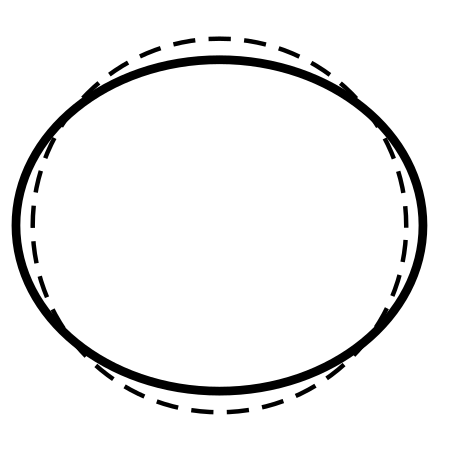
\includegraphics[height=3cm]{error_types/oval_error_schematic.png}
    \label{fig:oval_error_schematic}
}\\
\subfloat[周方向長周期誤差]{
    \includegraphics[height=3cm]{error_types/roundness_long_error_schematic.png}
    \label{fig:roundness_long_error_schematic}
}
\hspace{5mm}
\subfloat[周方向中周期誤差]{
    \includegraphics[height=3cm]{error_types/roundness_medium_error_schematic.png}
    \label{fig:roundness_medium_error_schematic}
}
\hspace{5mm}
\subfloat[周方向短周期誤差]{
    \includegraphics[height=3cm]{error_types/roundness_short_error_schematic.png}
    \label{fig:roundness_short_error_schematic}
}
\\

\subfloat[テーパ角誤差]{
    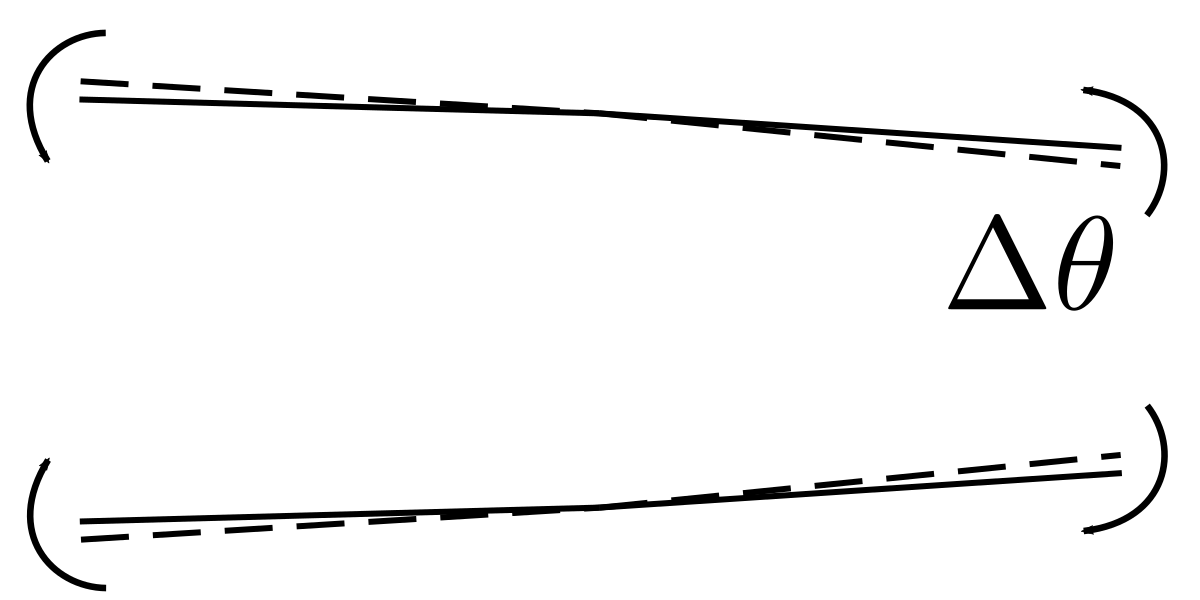
\includegraphics[height=3cm]{error_types/taper_error_schematic.png}
    \label{fig:taper_error_schematic}
}
\hspace{5mm}
\subfloat[光軸たわみ]{
    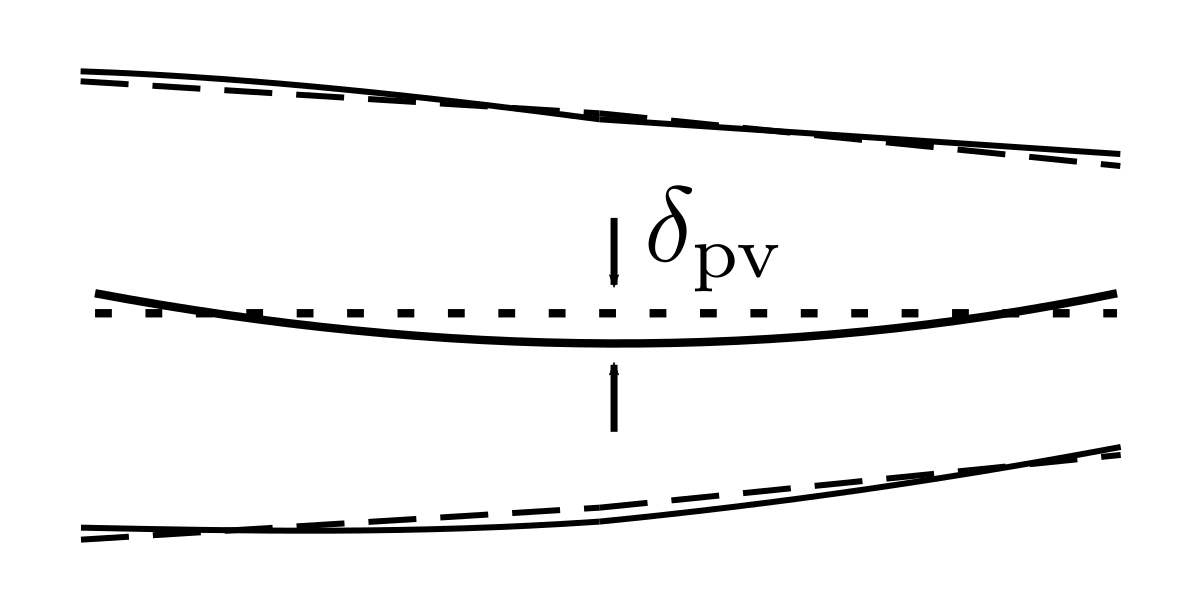
\includegraphics[height=3cm]{error_types/axis_deflection_schematic.png}
    \label{fig:axis_deflection_schematic}
}
\\

\subfloat[長手方向長周期形状誤差]{
    \includegraphics[height=3cm]{error_types/profile_long_error_schematic.png}
    \label{fig:profile_long_error_schematic}
}
\hspace{5mm}
\subfloat[長手方向中周期形状誤差]{
    \includegraphics[height=3cm]{error_types/profile_medium_error_schematic.png}
    \label{fig:profile_medium_error_schematic}
}
\\

\subfloat[長手方向短周期形状誤差]{
    \includegraphics[height=3cm]{error_types/profile_short_error_schematic.png}
    \label{fig:profile_short_error_schematic}
}

\caption[]{入力するミラー形状誤差の種類}
\label{fig:fwhm_explanation}
\end{figure}

\clearpage
% ================================================== %
% section
% ================================================== %
\newpage

\section{理想集光}
\label{chap2_ideal_focusing}

誤差入力を与える前に、誤差のない理想的なミラー形状に対する集光面強度分布を計算しておく。
表\ref{tb:ideal_simulation_params}に計算の条件を、またこれに対する可視光と硬X線に対する計算結果を図\ref{fig:ideal_simulation_visible}および図\ref{fig:ideal_simulation_xray}に示す。

% 計算条件の表
\begin{table}[!ht]
\begin{center}
  \caption[]{計算条件}
  \begin{tabular}{|c c c|} \hline
    項目 & 可視光 & 硬X線 \\ \hline
    エネルギー & 19.59 eV & 4.0 keV \\
    波長 & 632.8 nm & 0.310 nm \\
    焦点面画素サイズ & \SI{1.0}{\micro \metre} & 1.0 nm \\
    画素数 & \multicolumn{2}{c|}{$4096 \times 4096$} \\\hline
  \end{tabular}
  \label{tb:ideal_simulation_params}
\end{center}
\end{table}

% 計算結果の図
\begin{figure}[!ht]
\centering
\subfloat[焦点面強度分布]{
    \includegraphics[width=5cm]{ideal/focus_visible.png}
    \label{fig:ideal_focus_visible}
}
\subfloat[焦点面強度プロファイル ($y=0$)]{
    \includegraphics[width=8cm]{ideal/focus_profile_visible.png}
    \label{fig:ideal_focus_profile_visible}
}
\caption[]{可視光 (632.8 nm)}
\label{fig:ideal_simulation_visible}
\end{figure}

\begin{figure}[!ht]
\centering
\subfloat[焦点面強度分布]{
    \includegraphics[width=5cm]{ideal/focus_xray.png}
    \label{fig:ideal_focus_xray}
}
\subfloat[焦点面強度プロファイル ($y=0$)]{
    \includegraphics[width=8cm]{ideal/focus_profile_xray.png}
    \label{fig:ideal_focus_profile_xray}
}
\caption[]{硬X線 (4 keV)}
\label{fig:ideal_simulation_xray}
\end{figure}


これに対して、それぞれの波長に対するHPDおよびFWHMを表\ref{tb:ideal_focus_evaluation}に示す。
ただし、理想集光の場合は集光面強度分布が回転対象になっているため、FWHMは$y=0$の1本のプロファイルに対してのみ示す。

\begin{table}[!ht]
\begin{center}
  \caption{理想集光の場合のHPDおよびFWHM}
  \begin{tabular}{|c|c|c|} \hline
    項目 & 可視光(632.8nm) & 4keV \\ \hline
    HPD & 1.74 mm & \SI{0.87}{\micro \metre} \\
    FWHM & \SI{15.0}{\micro \metre} & 7.00 nm \\ \hline
  \end{tabular}
  \label{tb:ideal_focus_evaluation}
\end{center}
\end{table}

\clearpage
% ================================================== %
% section
% ================================================== %
\newpage

\section{X線に対する許容誤差量の解析}
\label{chap2_xray_allowed_error}

まず、4 keV のX線を光源とした場合について、入力する誤差量の変化に対するStrehl比およびHPDの変化を調べる。

% 直径誤差 -----------------------------------------
\subsection{(\ref{sub@fig:diameter_error_schematic}) 直径誤差}
\label{chap2_xray_diameter_error}

\begin{figure}[!ht]
\centering
\subfloat[Strehl比]{
    \includegraphics[width=7cm]{error_response/diameter/strehl.png}
    \label{fig:diameter_strehl}
}
\subfloat[HPD]{
    \includegraphics[width=7cm]{error_response/diameter/hpd.png}
    \label{fig:diameter_hpd}
}
\caption[]{(\ref{sub@fig:diameter_error_schematic}) 直径誤差}
\label{fig:diameter_allowed_error_analysis}
\end{figure}

% 真円度誤差 -----------------------------------------
\subsection{
    (\ref{sub@fig:oval_error_schematic})
    (\ref{sub@fig:roundness_long_error_schematic}) 
    (\ref{sub@fig:roundness_medium_error_schematic})
    (\ref{sub@fig:roundness_short_error_schematic})
    真円度誤差}
\label{chap2_xray_roundness_error}

真円度誤差についてのシミュレーション結果を示す。
まず、代表的な周期の誤差として、以下の4つについて示す。
\begin{itemize}
  \item (\ref{sub@fig:oval_error_schematic}) 二山誤差 (周期 $180^\circ$、 $\Delta r = \delta \sin 2\theta$)
  \item (\ref{sub@fig:roundness_long_error_schematic}) 長周期誤差 (周期 $40^\circ$、$\Delta r = \delta \sin 9\theta$)
  \item (\ref{sub@fig:roundness_medium_error_schematic}) 中周期誤差 (周期 $10^\circ$、$\Delta r = \delta \sin 36\theta$)
  \item (\ref{sub@fig:roundness_short_error_schematic}) 短周期誤差 (周期 $1^\circ$、$\Delta r = \delta \sin 360\theta$)
\end{itemize}

% 二山誤差 ----------------------------------------------------
\begin{figure}[!ht]
\centering
\subfloat[Strehl比]{
    \includegraphics[width=7cm]{error_response/oval/strehl.png}
    \label{fig:oval_strehl}
}
\subfloat[HPD]{
    \includegraphics[width=7cm]{error_response/oval/hpd.png}
    \label{fig:oval_hpd}
}
\caption[]{(\ref{sub@fig:oval_error_schematic}) 周方向二山誤差}
\label{fig:oval_allowed_error_analysis}
\end{figure}

% 長周期誤差 ----------------------------------------------------
\begin{figure}[!ht]
\centering
\subfloat[Strehl比]{
    \includegraphics[width=7cm]{error_response/roundness/strehl_40.png}
    \label{fig:roundness_long_strehl}
}
\subfloat[HPD]{
    \includegraphics[width=7cm]{error_response/roundness/hpd_40.png}
    \label{fig:roundness_long_hpd}
}
\caption[]{(\ref{sub@fig:roundness_long_error_schematic}) 周方向長周期誤差}
\label{fig:roundness_long_allowed_error_analysis}
\end{figure}

% 中周期誤差 ----------------------------------------------------
\begin{figure}[!ht]
\centering
\subfloat[Strehl比]{
    \includegraphics[width=7cm]{error_response/roundness/strehl_10.png}
    \label{fig:roundness_medium_strehl}
}
\subfloat[HPD]{
    \includegraphics[width=7cm]{error_response/roundness/hpd_10.png}
    \label{fig:roundness_medium_hpd}
}
\caption[]{(\ref{sub@fig:roundness_medium_error_schematic}) 周方向中周期誤差}
\label{fig:roundness_medium_allowed_error_analysis}
\end{figure}

% 短周期誤差 ----------------------------------------------------
\begin{figure}[!ht]
\centering
\subfloat[Strehl比]{
    \includegraphics[width=7cm]{error_response/roundness/strehl_1.png}
    \label{fig:roundness_short_strehl}
}
\subfloat[HPD]{
    \includegraphics[width=7cm]{error_response/roundness/hpd_1.png}
    \label{fig:roundness_short_hpd}
}
\caption[]{(\ref{sub@fig:roundness_short_error_schematic}) 周方向短周期誤差}
\label{fig:roundness_short_allowed_error_analysis}
\end{figure}

また、一定の誤差量に対して周期を変化させた際のPeak値およびHPDの変化を図\ref{fig:roundness_period_variety}に示す。

\begin{figure}[!ht]
\centering
\subfloat[Strehl比]{
    \includegraphics[width=7cm]{error_response/roundness/strehl_vs_period.png}
    \label{fig:roundness_strehl_vs_period}
}
\subfloat[HPD]{
    \includegraphics[width=7cm]{error_response/roundness/hpd_vs_period.png}
    \label{fig:roundness_strehl_vs_period}
}
\caption[]{真円度誤差の周期変化に対する応答}
\label{fig:roundness_period_variety}
\end{figure}


% テーパ角 -----------------------------------------
\subsection{(\ref{sub@fig:taper_error_schematic}) テーパ角}
\label{chap2_xray_taper_error}

\begin{figure}[!ht]
\centering
\subfloat[Strehl比]{
    \includegraphics[width=7cm]{error_response/taper/strehl.png}
    \label{fig:taper_strehl}
}
\subfloat[HPD]{
    \includegraphics[width=7cm]{error_response/taper/hpd.png}
    \label{fig:taper_hpd}
}
\caption[]{(\ref{sub@fig:taper_error_schematic}) テーパ角}
\label{fig:axis_deflection_allowed_error_analysis}
\end{figure}


% 光軸たわみ -----------------------------------------
\subsection{(\ref{sub@fig:axis_deflection_schematic}) 光軸たわみ}
\label{chap2_xray_axis_deflection}

\begin{figure}[!ht]
\centering
\subfloat[Strehl比]{
    \includegraphics[width=7cm]{error_response/axis_deflection/strehl.png}
    \label{fig:axis_deflection_strehl}
}
\subfloat[HPD]{
    \includegraphics[width=7cm]{error_response/axis_deflection/hpd.png}
    \label{fig:axis_deflection_hpd}
}
\caption[]{(\ref{sub@fig:axis_deflection_schematic}) 光軸たわみ}
\label{fig:axis_deflection_allowed_error_analysis}
\end{figure}

% 長手プロファイル誤差 -----------------------------------

% 長周期誤差 ----------------------------------------------------
\begin{figure}[!ht]
\centering
\subfloat[Strehl比]{
    \includegraphics[width=7cm]{error_response/meridional/strehl_100.png}
    \label{fig:meridional_long_strehl}
}
\subfloat[HPD]{
    \includegraphics[width=7cm]{error_response/meridional/hpd_100.png}
    \label{fig:meridional_long_hpd}
}
\caption[]{(\ref{sub@fig:profile_long_error_schematic}) 長手方向長周期誤差}
\label{fig:meridional_long_allowed_error_analysis}
\end{figure}

% 中周期誤差 ----------------------------------------------------
\begin{figure}[!ht]
\centering
\subfloat[Strehl比]{
    \includegraphics[width=7cm]{error_response/meridional/strehl_10.png}
    \label{fig:meridional_medium_strehl}
}
\subfloat[HPD]{
    \includegraphics[width=7cm]{error_response/meridional/hpd_10.png}
    \label{fig:meridional_medium_hpd}
}
\caption[]{(\ref{sub@fig:profile_medium_error_schematic}) 長手方向中周期誤差}
\label{fig:meridional_medium_allowed_error_analysis}
\end{figure}

% 短周期誤差 ----------------------------------------------------
\begin{figure}[!ht]
\centering
\subfloat[Strehl比]{
    \includegraphics[width=7cm]{error_response/meridional/strehl_1.png}
    \label{fig:meridional_short_strehl}
}
\subfloat[HPD]{
    \includegraphics[width=7cm]{error_response/meridional/hpd_1.png}
    \label{fig:meridional_short_hpd}
}
\caption[]{(\ref{sub@fig:profile_short_error_schematic}) 長手方向短周期誤差}
\label{fig:meridional_short_allowed_error_analysis}
\end{figure}

また、一定の誤差量に対して周期を変化させた際のPeak値およびHPDの変化を図\ref{fig:meridional_period_variety}に示す。

\begin{figure}[!ht]
\centering
\subfloat[Strehl比]{
    \includegraphics[width=7cm]{error_response/meridional/strhel_vs_period.png}
    \label{fig:meridional_strehl_vs_period}
}
\subfloat[HPD]{
    \includegraphics[width=7cm]{error_response/meridional/hpd_vs_period.png}
    \label{fig:meridional_strehl_vs_period}
}
\caption[]{長手プロファイル誤差の周期変化に対する応答}
\label{fig:meridional_period_variety}
\end{figure}


% まとめ -----------------------------------------
\subsection{総合的な解析}
\label{chap2_xray_error_response_summary}

\begin{table}[!ht]
\begin{center}
  \caption{形状誤差の種類ごとの許容値}
  \begin{tabular}{|c|c|c|} \hline
    形状誤差の種類 & Strehl比0.8 & HPD 0.5 秒角 \\ \hline
    (\ref{sub@fig:diameter_error_schematic}) 直径誤差 & 0.0 mm & 0.0 mm \\
    (\ref{sub@fig:oval_error_schematic}) 周方向二山誤差 & 2.0 nm & \SI{1.5}{\micro \metre} \\ \hline
  \end{tabular}
  \label{tb:xray_allowed_error}
\end{center}
\end{table}

\begin{comment}
また、これらに対応する集光面強度分布を示す。

\begin{figure}[!ht]
\centering
\subfloat[焦点面強度分布]{
    \includegraphics[width=5cm]{ideal/focus_xray.png}
    \label{fig:ideal_focus_xray}
}
\subfloat[焦点面強度プロファイル ($y=0$)]{
    \includegraphics[width=8cm]{ideal/focus_profile_xray.png}
    \label{fig:ideal_focus_profile_xray}
}
\caption[]{硬X線 (4 keV)}
\label{fig:xray_just_allowed_focus}
\end{figure}
\end{comment}


\clearpage
% ================================================== %
% section
% ================================================== %
\newpage

\section{可視光光源を用いた場合の位相分布の解析}
\label{chap2_error_response_visible}



\clearpage
% ================================================== %
% section
% ================================================== %
\newpage
\section{収差解析}
\label{chap2_simulation_zernike_analysis}

\ref{chap2_simulation_error_response}節では、ミラー加工において生じる様々な誤差を紹介するとともに、その誤差入力についてのシミュレーションを行った。
本節では、\ref{chap3}章で述べる位相回復によって得られた波面情報から各誤差への分解を行うための解析方法について検討する。

\subsection{Zernike収差}

\subsection{輪帯状の位相分布に対するZernike収差}


\subsection{各誤差に起因する収差の解析}



\section{結言}
\label{chap2_conclusion}



%%%%%%%%%%%%%%%%%%%%%%%%%%%%%%%%%%%%%%%%%%%%%%%%%%%%%%%%%%%%%%%%%%%%%%%%%%%%%
%%% Local Variables:
%%% mode: katex
%%% TeX-master: "../thesis"
%%% End:
